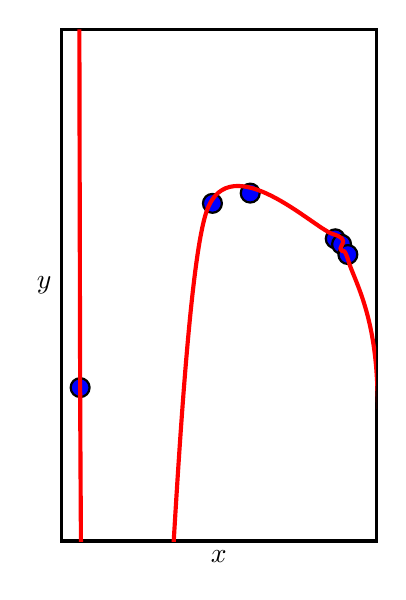
\begin{tikzpicture}
  \tikzset{
  data_pic/.pic={
    % plot frame
    \draw[line width=1.2pt] (0,0) rectangle (4,6.5);

    % data points
    \filldraw[blue, draw=black, line width=0.8pt] (0.24,1.95) circle (0.12);
    \filldraw[blue, draw=black, line width=0.8pt] (1.92,4.29) circle (0.12);
    \filldraw[blue, draw=black, line width=0.8pt] (2.40,4.42) circle (0.12);
    \filldraw[blue, draw=black, line width=0.8pt] (3.48,3.84) circle (0.12);
    \filldraw[blue, draw=black, line width=0.8pt] (3.56,3.77) circle (0.12);
    \filldraw[blue, draw=black, line width=0.8pt] (3.64,3.64) circle (0.12);

    % characteristic coordinates of plot
    \coordinate (-oo) at (0, 0);
    \coordinate (-top) at (2, 6.5);
    \coordinate (-bottom) at (2, 0);
    \coordinate (-left) at (0, 3.25);
  }
}

  % img
  \pic (pic_o) at (11, 0) {data_pic};
  \begin{scope}[shift={(pic_o-oo)}]
    \clip (0,0) rectangle (4,6.5);
    \draw[
      red,
      line width=1.5pt
    ] plot[smooth] coordinates {
      (0.23,6.5)
      (0.24,2.0)
      (0.25,0.0)
      (0.26,-2.0)
      (1.30,-0.1)
      (1.30,-2.0)
      (1.85,4.2)
      (3.45,3.90)
      (3.55,3.70)
      (3.65,3.55)
      (4.00,2.2)
      (4.10,-2.0)
    };
  \end{scope}

  % % titles
  % \draw (pic_o-top) node[anchor=south] {Zbyt złożony model};

  % axis
  \draw (pic_o-bottom) node[anchor=north] {$x$};
  \draw (pic_o-left) node[anchor=east] {$y$};
\end{tikzpicture}